\documentclass[]{article}

\usepackage{amsmath}  % AMS math package
\usepackage{amssymb}  % AMS symbol package
\usepackage{bm}       % bold math
\usepackage{graphicx} % Include figure files
\usepackage{dcolumn}  % Align table columns on decimal point
\usepackage{caption}
\usepackage{subcaption}
\usepackage{hyperref}
%\usepackage{multirow} % Multirow/column tables

\begin{document}

\title{PHY 905 Project 1: Monte Carlo simulation of the 2-D ferromagnetic Ising model}

\author{Steve Hughey}

\date{\today}

\maketitle

\begin{abstract}
A simple Fortran implementation of the Metropolis algorithm for Monte Carlo simulation of the Ising model of ferromagnetism is described. Results are presented for energy and magnetization over a range of temperature.
\end{abstract}

\section{\label{sec:intro}Introduction}

In statistical mechanics, the Ising model is a mathematical model of ferromagnetism in a $d$-dimensional lattice. In this document, we consider the case $d=2$. The magnetization of the lattice depends on the values of the spins at each lattice site. Since the allowed spin at any lattice site $i$ must belong to the set $\left\lbrace -1, 1 \right\rbrace$, there are $2^N$ allowable lattice states, where $N$ is the total number of lattice sites. As $N$ increases much beyond 10, computation of every single allowable state becomes intractable on a computer. Monte Carlo simulation of the Ising model, known as the Metropolis algorithm, allows us to the study the behavior of the system as the temperature of the system is varied.

\subsection{\label{sec:ising}Ising model basics}

The energy $H$ of the $N_x \times N_y$ lattice is a sum over all nearest neighbor spin products, multiplied by an interaction strength $J$:
\begin{align}
H =& -J \sum_{<i,j>} s_i s_j
\end{align}

The magnetization $M$ of the lattice in a given state is computed as a sum over all spins in the lattice, normalized by the number of lattice points:

\begin{align}
M =& \frac{1}{N_x N_y}\sum_{i} s_i
\end{align}

In this document, we are interested only in the energy and magnetization of the system in a given state.

\section{\label{sec:imp}Implementation}

At each step of the Monte Carlo iteration, a lattice site $i$ is chosen at random. The spin $s_i$ of this site is negated with probability $e^{-\Delta E_i / k_B T}$. Boltzmann's constant $k_B$ is set equal to $1$ for convenience, so that the temperature $T$ is measured in units of $k_B$.

The change in energy $\Delta E_i$ due to negating the spin of a single point $i$ in the lattice is computed as the sum of $i$'s nearest neighbor spins multiplied by the hypothetical new value of the spin $s_i$ and the interaction strength $J$:

\begin{align}
\Delta E_i =& J s_i \sum_{<j>} s_j
\end{align}

The change in magnetization due to a flipped spin is twice the value of the new spin $s_i$, divided by the total number of lattice sites.

\subsection{\label{sec:alg}Metropolis Algorithm}

The Metropolis algorithm comprises the following steps:

\begin{enumerate}
 \item Choose a temperature $T$ and maximum iteration count $N_{iter}$
 \item Initialize lattice with all spins up
 \item Compute initial total energy $H$ and magnetization $M$
 \item Iterate $N_{iter}$ times:
 \begin{enumerate}
  \item Select a lattice site $i$ at random
  \item Compute the change in energy $\Delta E_i$ due to negating the spin at lattice site $i$
  \item If $\Delta E_i < 0$, retain the flipped spin value at site $i$, compute the change in magnetization, and update total energy and magnetization
  \item Otherwise ($\Delta E_i > 0$), retain the flipped spin value at site $i$ with probability $e^{-\Delta E_i / k_B T}$; if retained, update energy and magnetization
 \end{enumerate}
\end{enumerate}

\section{\label{sec:res}Results}

A Fortran code was written which implements the 2D Ising model. The source code can be found in the \href{https://github.com/hugheyst/ising}{GitHub repository}. The results in this section were obtained using a $(N_x,N_y) = 50 \times 50$ lattice with all spins up as the initial state. Plots with temperature on the horizontal axis were obtained by averaging the final 50,000 values of energy and magnetization from an iteration with $N_{iter} = 1 \times 10^6$.

\begin{figure}[ht!]
 \centering
 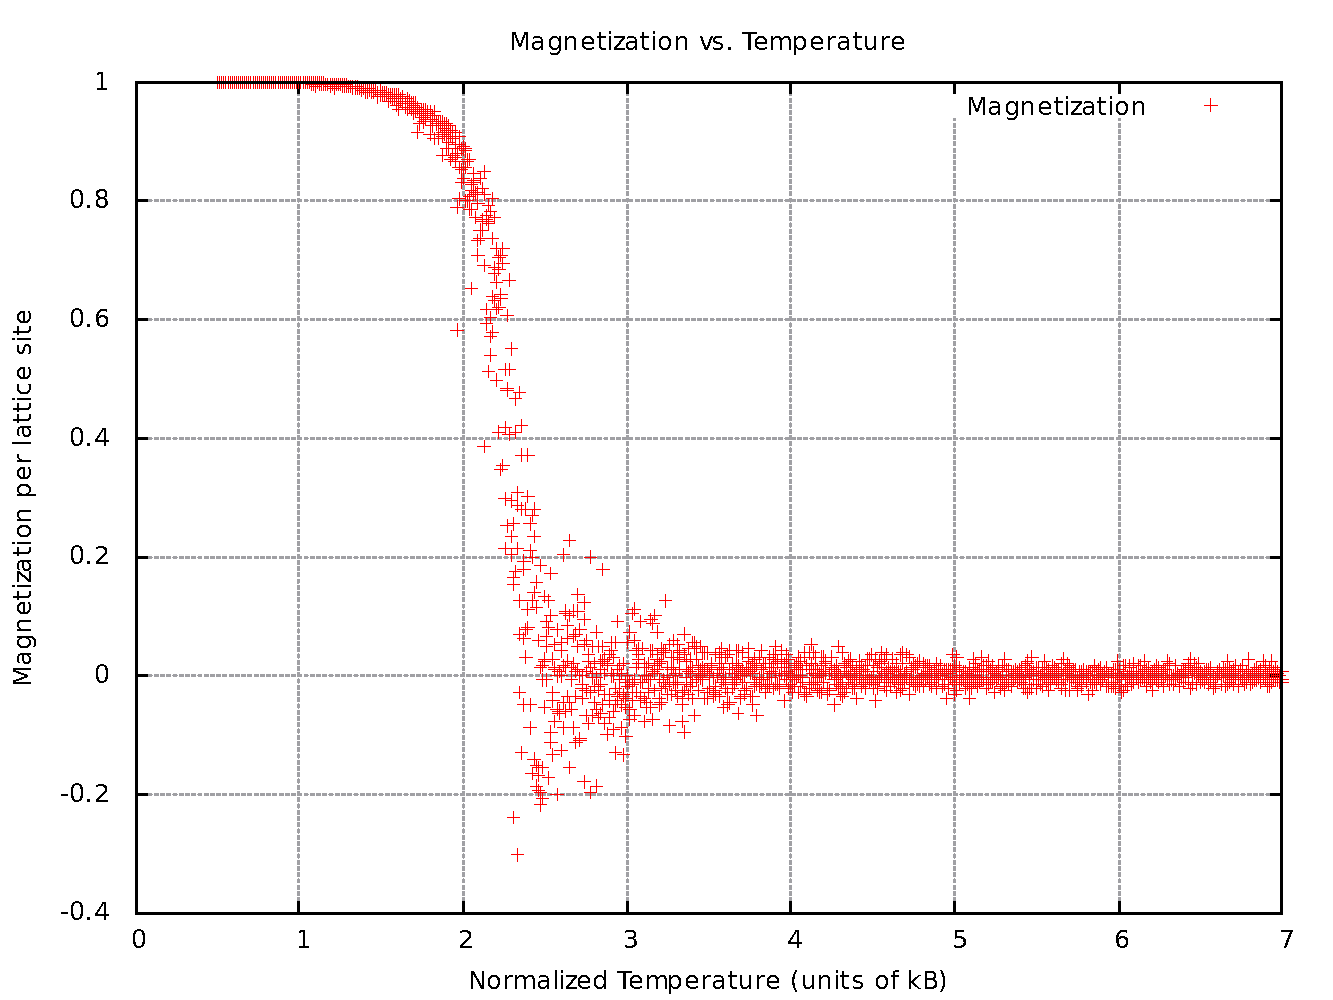
\includegraphics[width=\linewidth]{figures/mag_vs_temp.pdf}
 \caption{Magnetization per lattice site from $T=0.5$ to $T=7$. Values computed by averaging final 50000 Monte Carlo iterations per temperature value.}
 \label{fig:mag_vs_temp}
\end{figure}

Fig. \ref{fig:mag_vs_temp} shows the magnetization per lattice site over a range of temperatures. At low temperatures, there is not enough thermal energy in the system to flip many spins from their initial $+1$ state. Almost all of the spins remain aligned up to about $T=2$, an example of which can be seen in Fig. \ref{fig:spin_t_eq_2}. The magnetization thus remains strong until the critical temperature is approached, just over $T=2.25$, after which the magnetization tends toward zero. Zero magnetization implies that there are equal numbers of positive and negative spins in the lattice. Examples of this chaotic post-critical arrangement can be seen in Figs. \ref{fig:spin_t_eq_2p3} - \ref{fig:spin_t_eq_3}.

\begin{figure}[ht!]
 \centering
 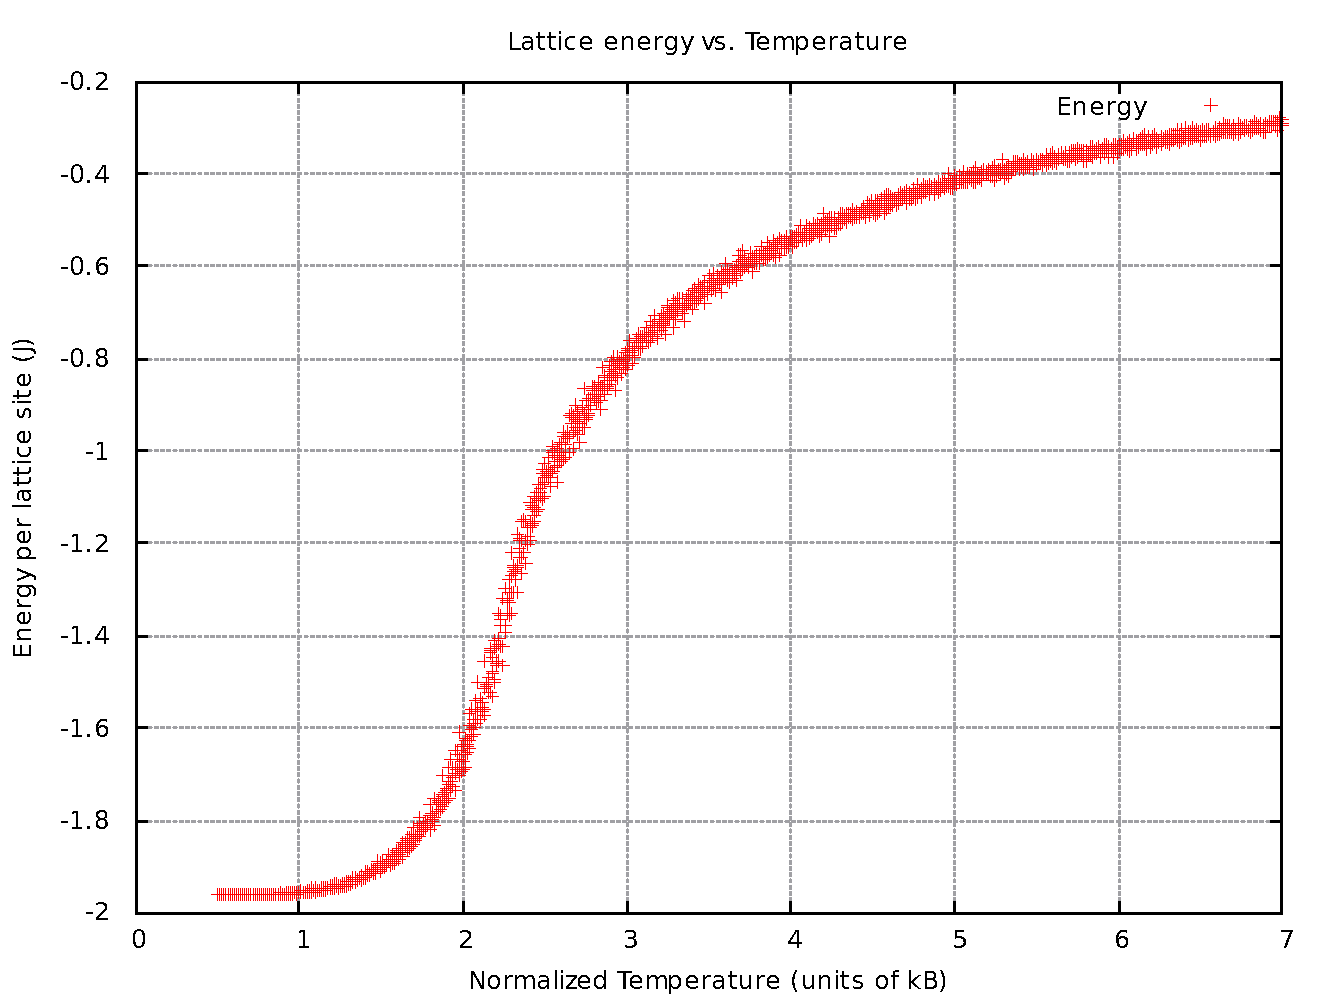
\includegraphics[width=\linewidth]{figures/energy_vs_temp.pdf}
 \caption{Lattice energy per lattice site from $T=0.5$ to $T=7$. Values computed by averaging final 50000 Monte Carlo iterations per temperature value.}
 \label{fig:energy_vs_temp}
\end{figure}

As the temperature increases, we expect that the total energy of the system will increase due to an increase in thermal energy. This phenomenon is demonstrated in Fig. \ref{fig:energy_vs_temp} over the range $T=0.5$ to $T=7$. A sharp increase in energy is observed near the critical temperature $T \approx 2.25$. This corresponds to a phase change, which explains the precipitous drop in magnetization at the same temperature. States with high energy have more chaotic configurations, and thus lack the strong alignment which yields the high magnetization of low-energy states.

\begin{figure}[ht!]
 \centering
 \begin{subfigure}[b]{0.3\linewidth}
  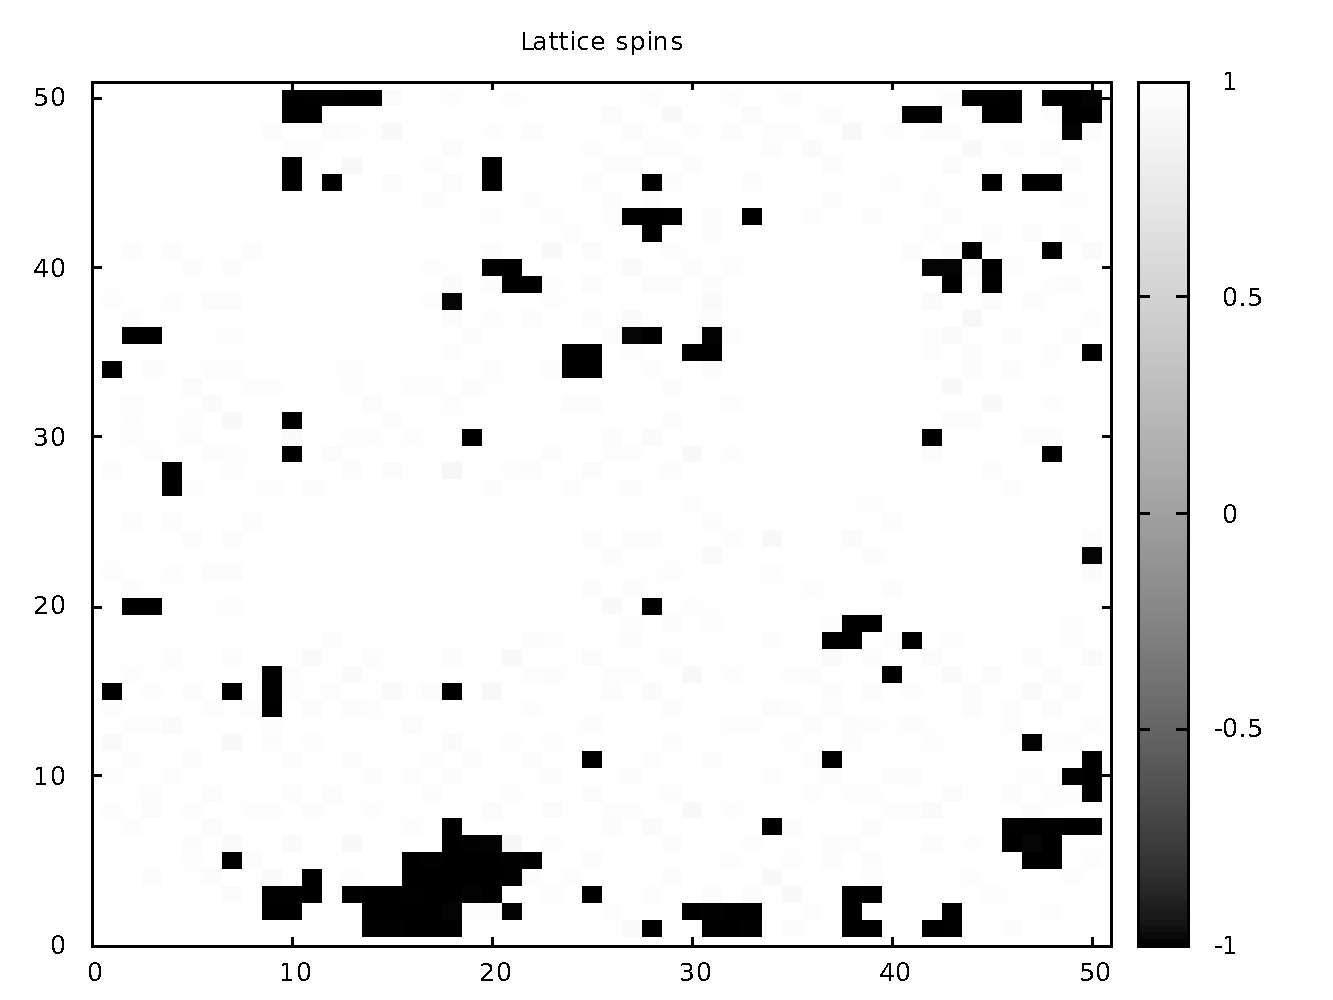
\includegraphics[width=\textwidth]{figures/spin_T_eq_2.pdf}
  \caption{$T=2$}
  \label{fig:spin_t_eq_2}
 \end{subfigure}
 \begin{subfigure}[b]{0.3\linewidth}
  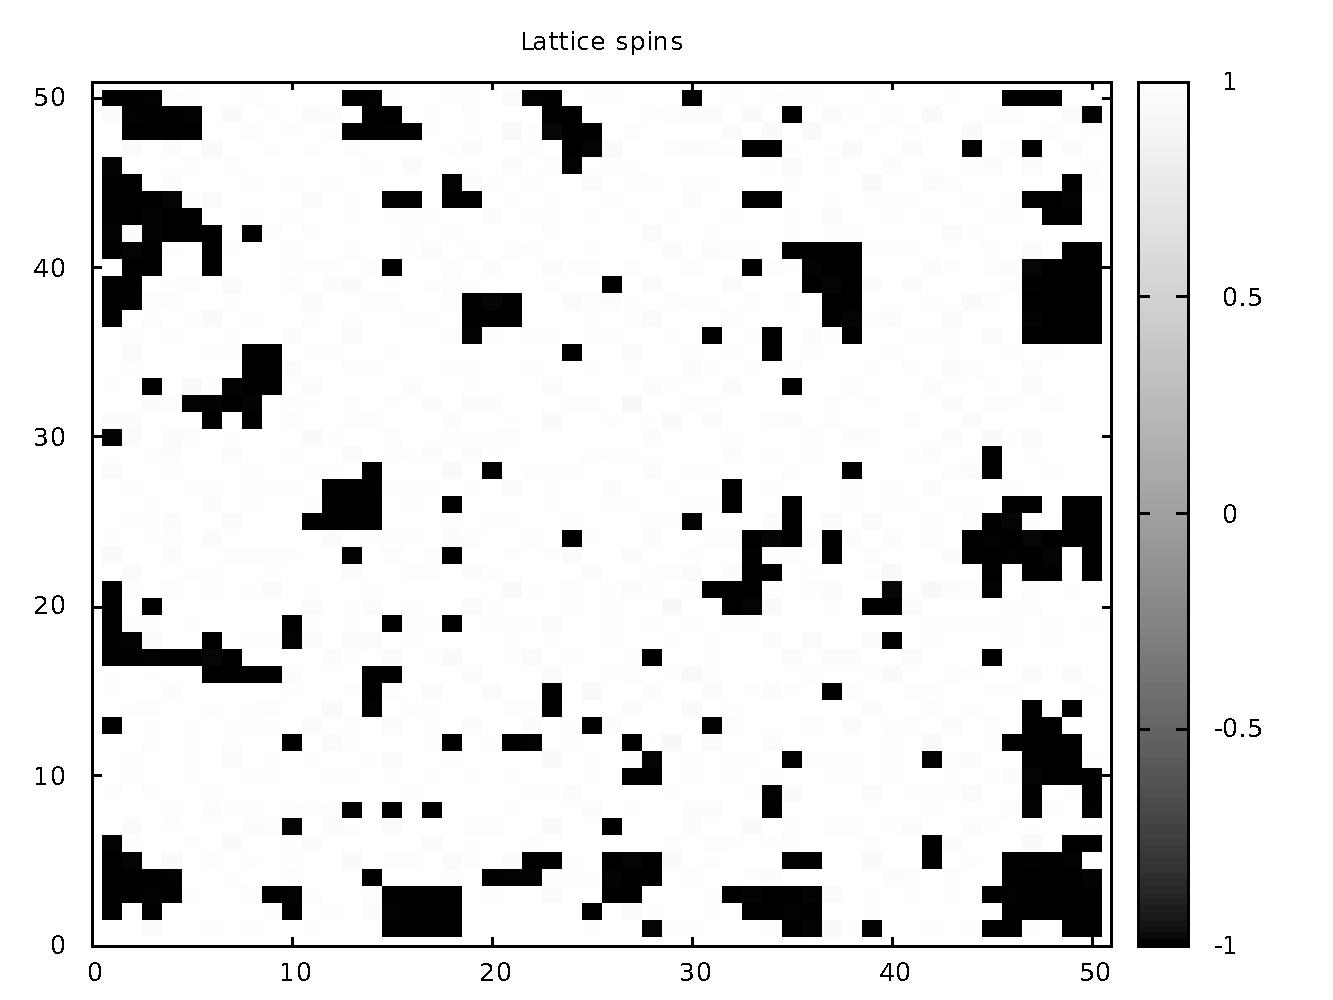
\includegraphics[width=\textwidth]{figures/spin_T_eq_2p2.pdf}
  \caption{$T=2.2$}
  \label{fig:spin_t_eq_2p2}
 \end{subfigure}
 \begin{subfigure}[b]{0.3\linewidth}
  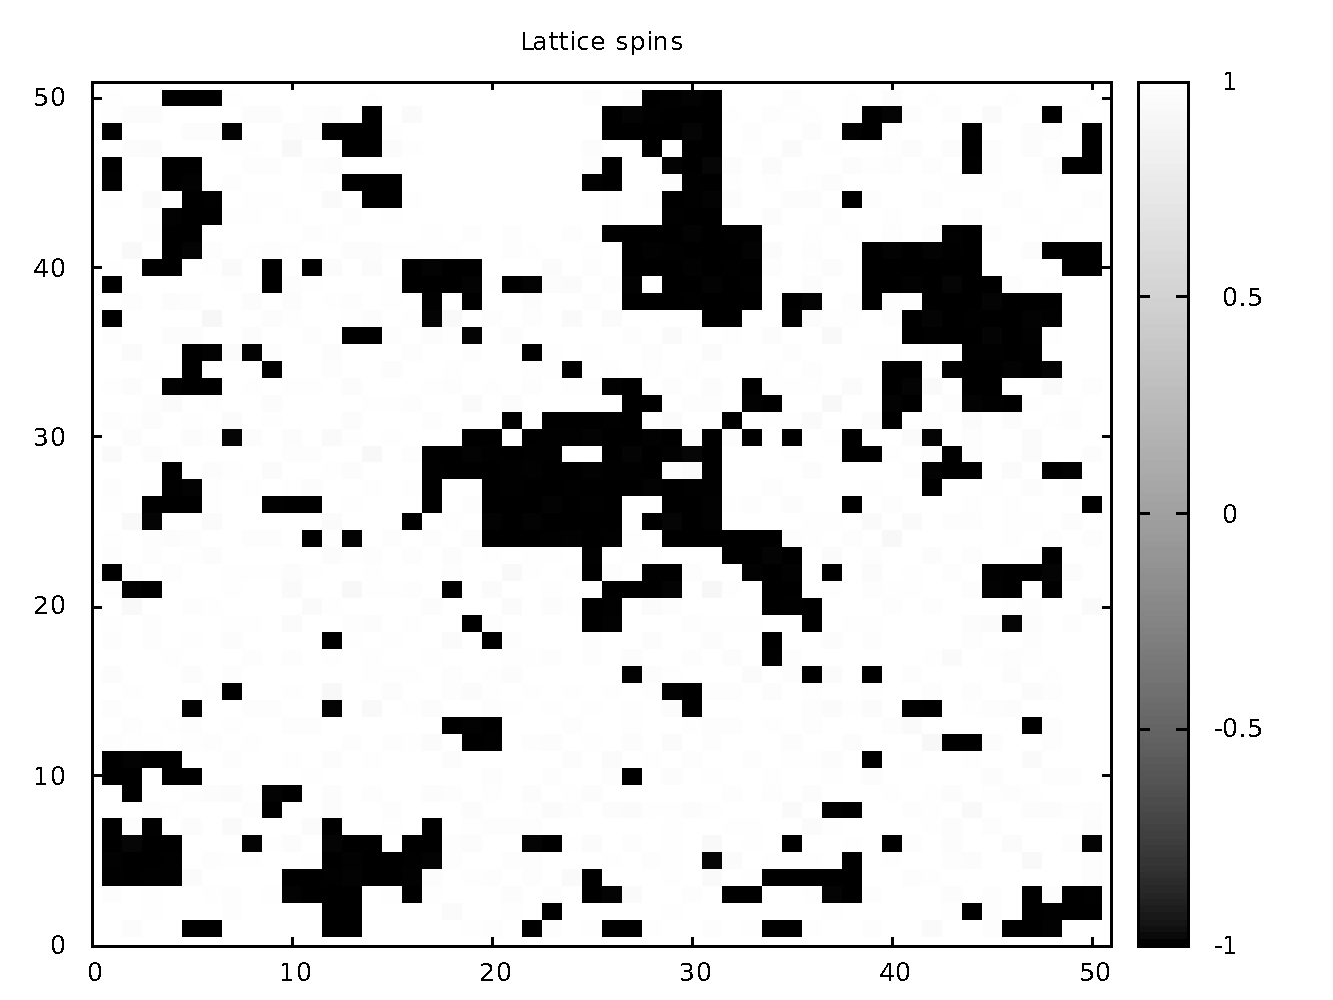
\includegraphics[width=\textwidth]{figures/spin_T_eq_2p25.pdf}
  \caption{$T=2.25$}
  \label{fig:spin_t_eq_2p25}
 \end{subfigure}
 
  \begin{subfigure}[b]{0.3\linewidth}
  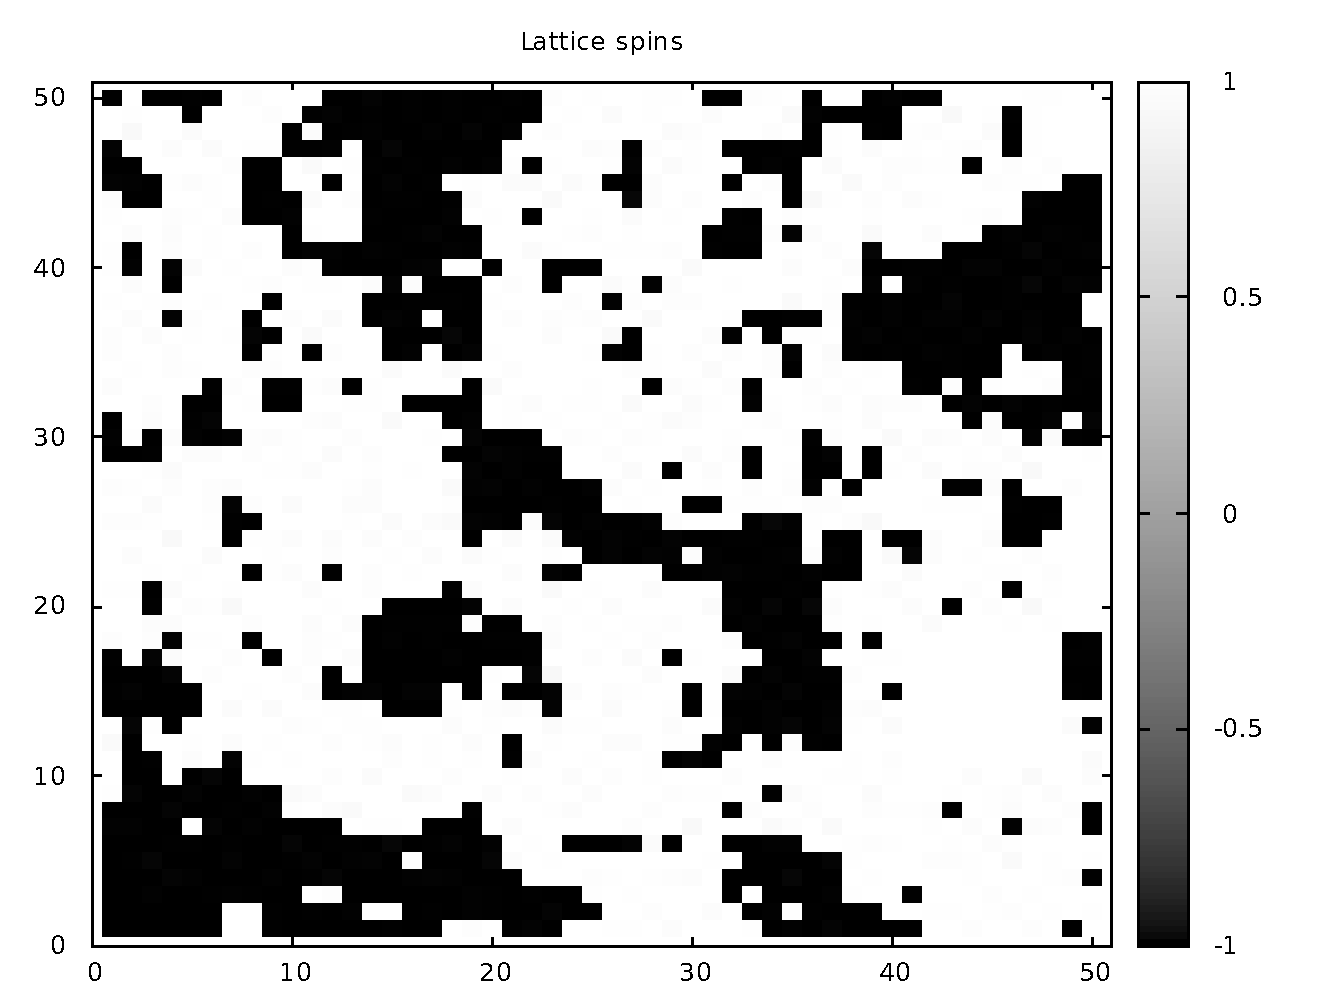
\includegraphics[width=\textwidth]{figures/spin_T_eq_2p3.pdf}
  \caption{$T=2.3$}
  \label{fig:spin_t_eq_2p3}
 \end{subfigure}
 \begin{subfigure}[b]{0.3\linewidth}
  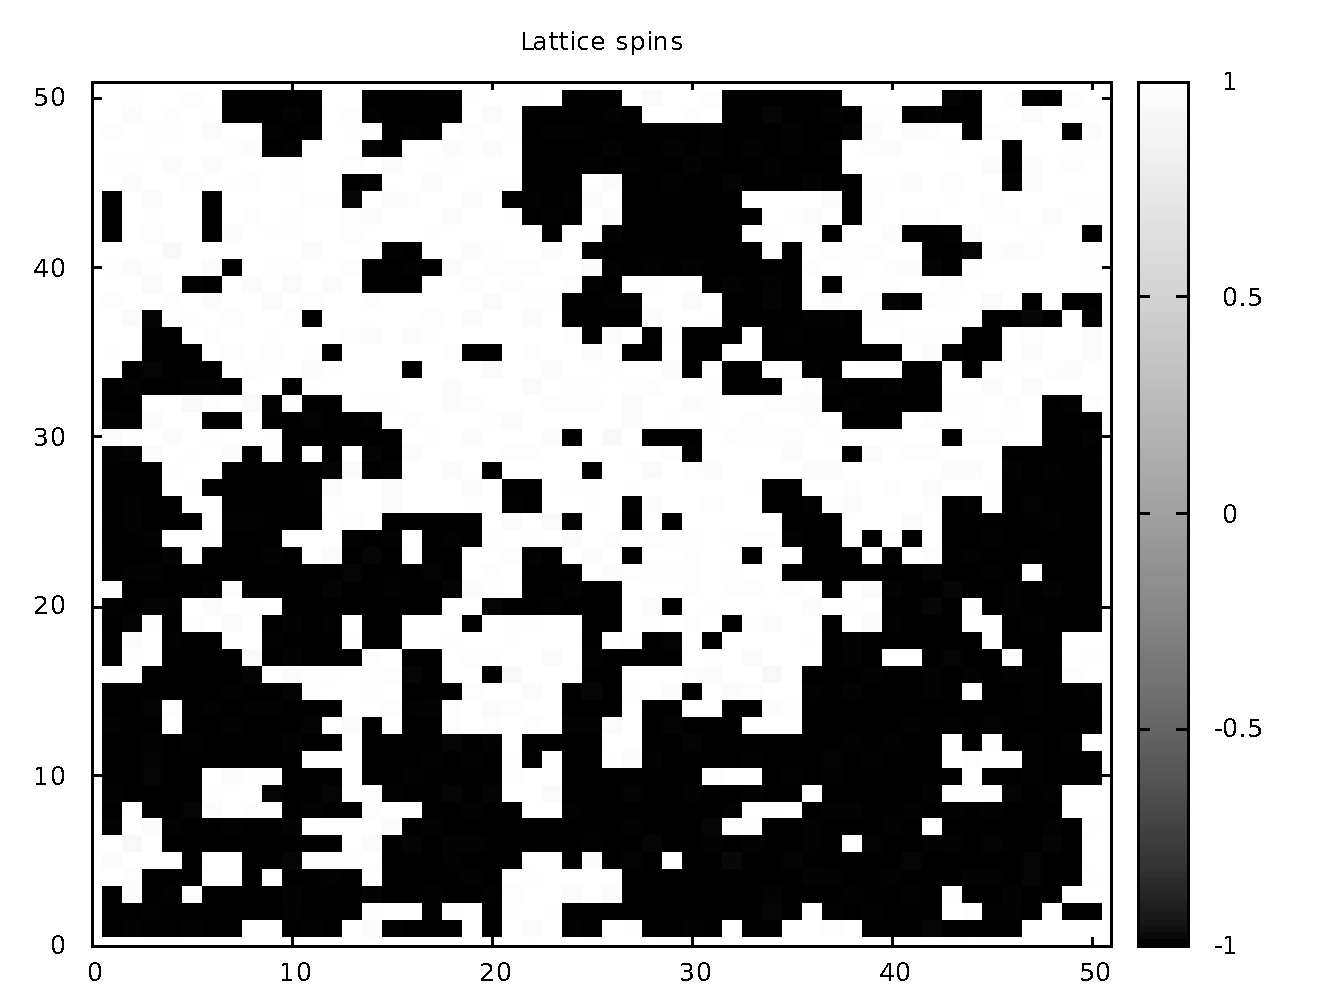
\includegraphics[width=\textwidth]{figures/spin_T_eq_2p5.pdf}
  \caption{$T=2.5$}
  \label{fig:spin_t_eq_2p5}
 \end{subfigure}
 \begin{subfigure}[b]{0.3\linewidth}
  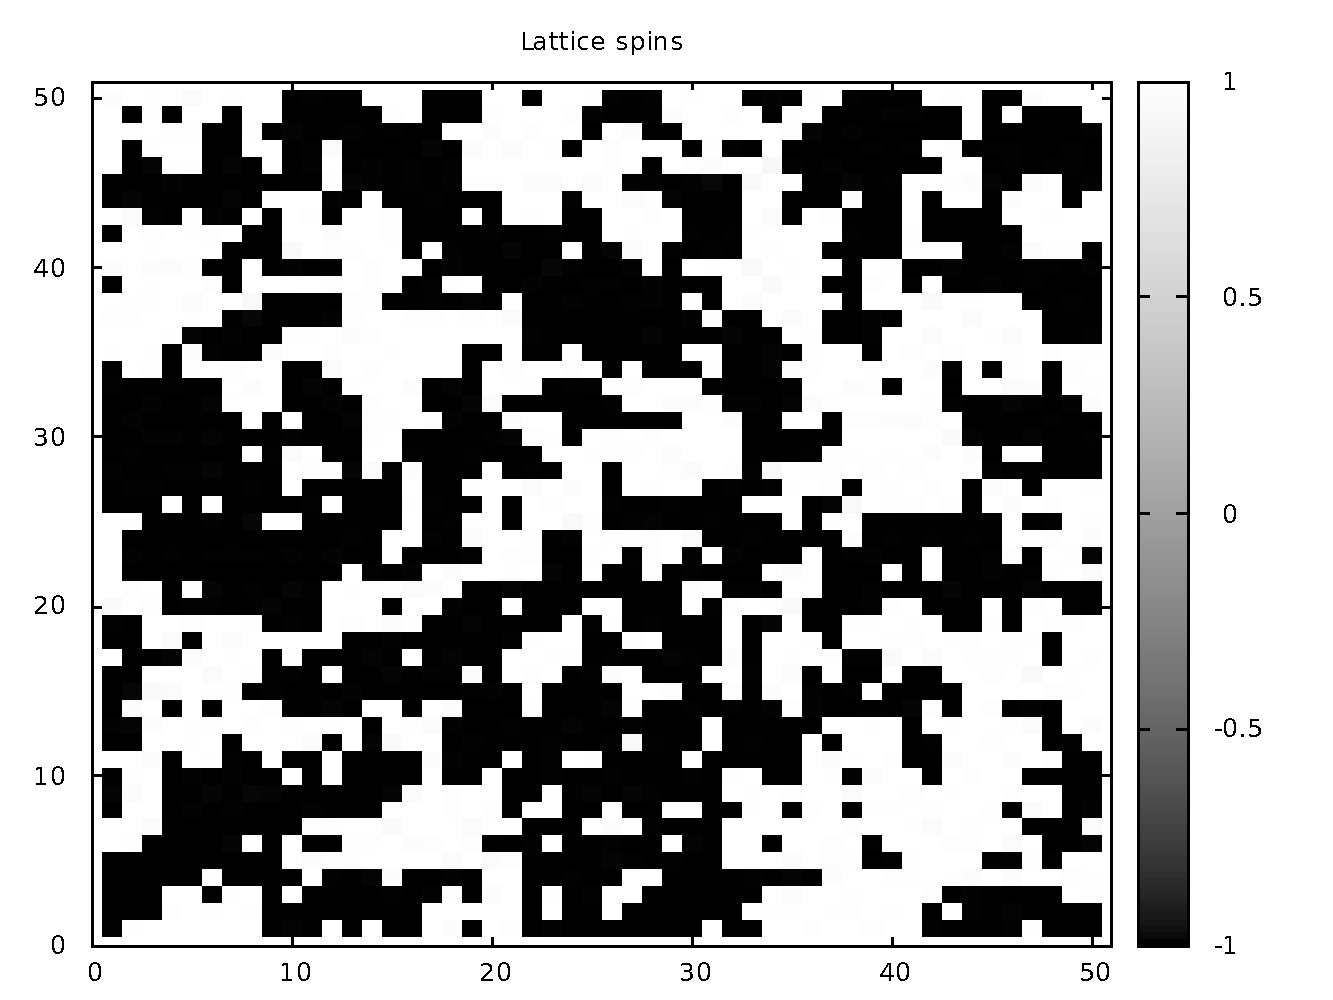
\includegraphics[width=\textwidth]{figures/spin_T_eq_3.pdf}
  \caption{$T=3$}
  \label{fig:spin_t_eq_3}
 \end{subfigure}
 
 \caption{Example late-time lattice states for various temperatures.}
 \label{fig:spins}
\end{figure}

A selection of example lattice configurations for various temperatures below, near, and above the critical temperature are shown in Fig. \ref{fig:spins}. Each of these configurations was sampled from the final state of a Monte Carlo iteration, so they can be considered representative examples of their individual energies. As the temperature of the lattice increases, the spin distribution becomes clearly more chaotic, and at the upper end of the chosen temperature range it is reasonable to estimate visually that the number of up and down spins in the lattice are roughly equal, corresponding to approximately zero magnetization. These results are reflective of the energy and magnetization data in Figs. \ref{fig:energy_vs_temp} and \ref{fig:mag_vs_temp}, respectively.

\section{Conclusion}

In this document, the Ising model of ferromagnetism and the Metropolis algorithm for numerical simulation of the model were briefly summarized. Results from a Fortran implementation of the Metropolis algorithm were presented and discussed. The observed trends in the data were found to be consistent with known physics.

\end{document}